We connect the two confirmations with two readings, and we take both from the same repeated branches rather than from a new experiment. The first is how much per-task signal the menu carries. We give a per-task selector one complete independent draw of every arm and score it on the other draw. It reaches 50.80\% on triggered prefixes against 49.09\% for the best arm in hindsight, the warning, a margin of 1.71 points; under the scheduled rule the same quantities are 52.50\% and 53.33\% for the relocation message, a margin of $-$0.83 points. A trigger exists on 497/593 tasks, against 540/593 that reach the scheduled checkpoint on the same identities, so the event rule does not open its room by offering more chances to act. Relative to continuation the arm means are the warning 0.20, replanning $-$0.70, the one-step rollback $-$1.81, the three-step rollback $-$3.42, the relocation message $-$0.80 percentage points, so the menu is not interchangeable: the three-step rollback is the costliest arm on average and the warning the least costly. An average cost is not a verdict on any prefix, which is the distinction a controller is asked to make. Conditioning the decision on a public failure signal is what opens prefix-level room for a controller; a larger learner at the earlier decision point does not. The paired rules make that reading falsifiable, because the menu and the identities are the same on both. Where the reading is negative, average repair is what pays for a rule fitted at a different decision point: under the scheduled rule cross-draw control adds 0.51 points over continuation, while the failure-risk detector fires on 86.1\% of prefixes and adds 3.71, which is close to the menu's unconditional effect rather than a prefix-level one. Where the instrument reports positive room the ordering reverses, and cross-draw control leads that detector by 1.85 points. The decision point, not the menu, decides what a controller has to condition on.

The second reading is how much of the same-draw gap is mechanical. We permute the recorded action and draw labels within each task, which fixes the continuation noise level and removes any action structure. Under the event rule the observed gap is 17.37 points over planned tasks and 20.72 points over eligible prefixes, against an exchangeable-label floor of 23.72 points ([21.43, 25.96]). The gap tracks continuation noise, which is why it is reported as an estimate rather than tested.

\begin{figure}[t]
\centering
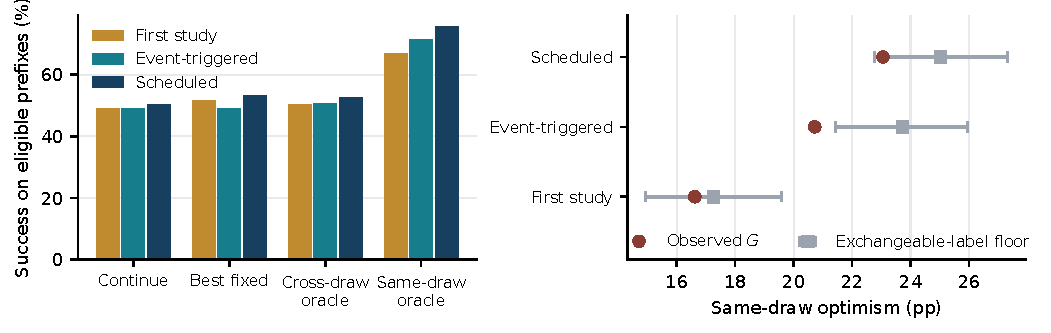
\includegraphics[width=0.9\linewidth]{figures/headroom.pdf}
\caption{How much per-task signal the decision point and the action menu carry, and how much same-draw optimism is mechanical. Left: success on eligible prefixes for continuation, the best arm in hindsight, and per-task selectors scored across and within draws, for the first study's scheduled panel and both rules of the second. Right: observed same-draw optimism against the within-task exchangeable-label reference.}
\label{fig:headroom}
\end{figure}

